	
	A continuación se presenta el \emph{script} con la implementación del algorítmo. 
	\lstinputlisting[linerange=Implementacion-fin]{ej_3.m}

	En la Figura \ref{fig:ej3} se expone la convergencia de los coeficientes en función de la cantidad de muestras (tiempo). Se puede ver que para más de 300 muestras, la estimación es correcta. Sin embargo al presentarse ruido en la medición de la salida, la estimación fluctúa alrededor del valor correcto. 
	\Juan{No estoy seguro que esté taaan bien}
	Si la incertidumbre de la medición es muy grande, la estimación tardará más en converger y oscilará en un rango mayor entorno al verdadero.

	\begin{figure}[h!]
		\centering
		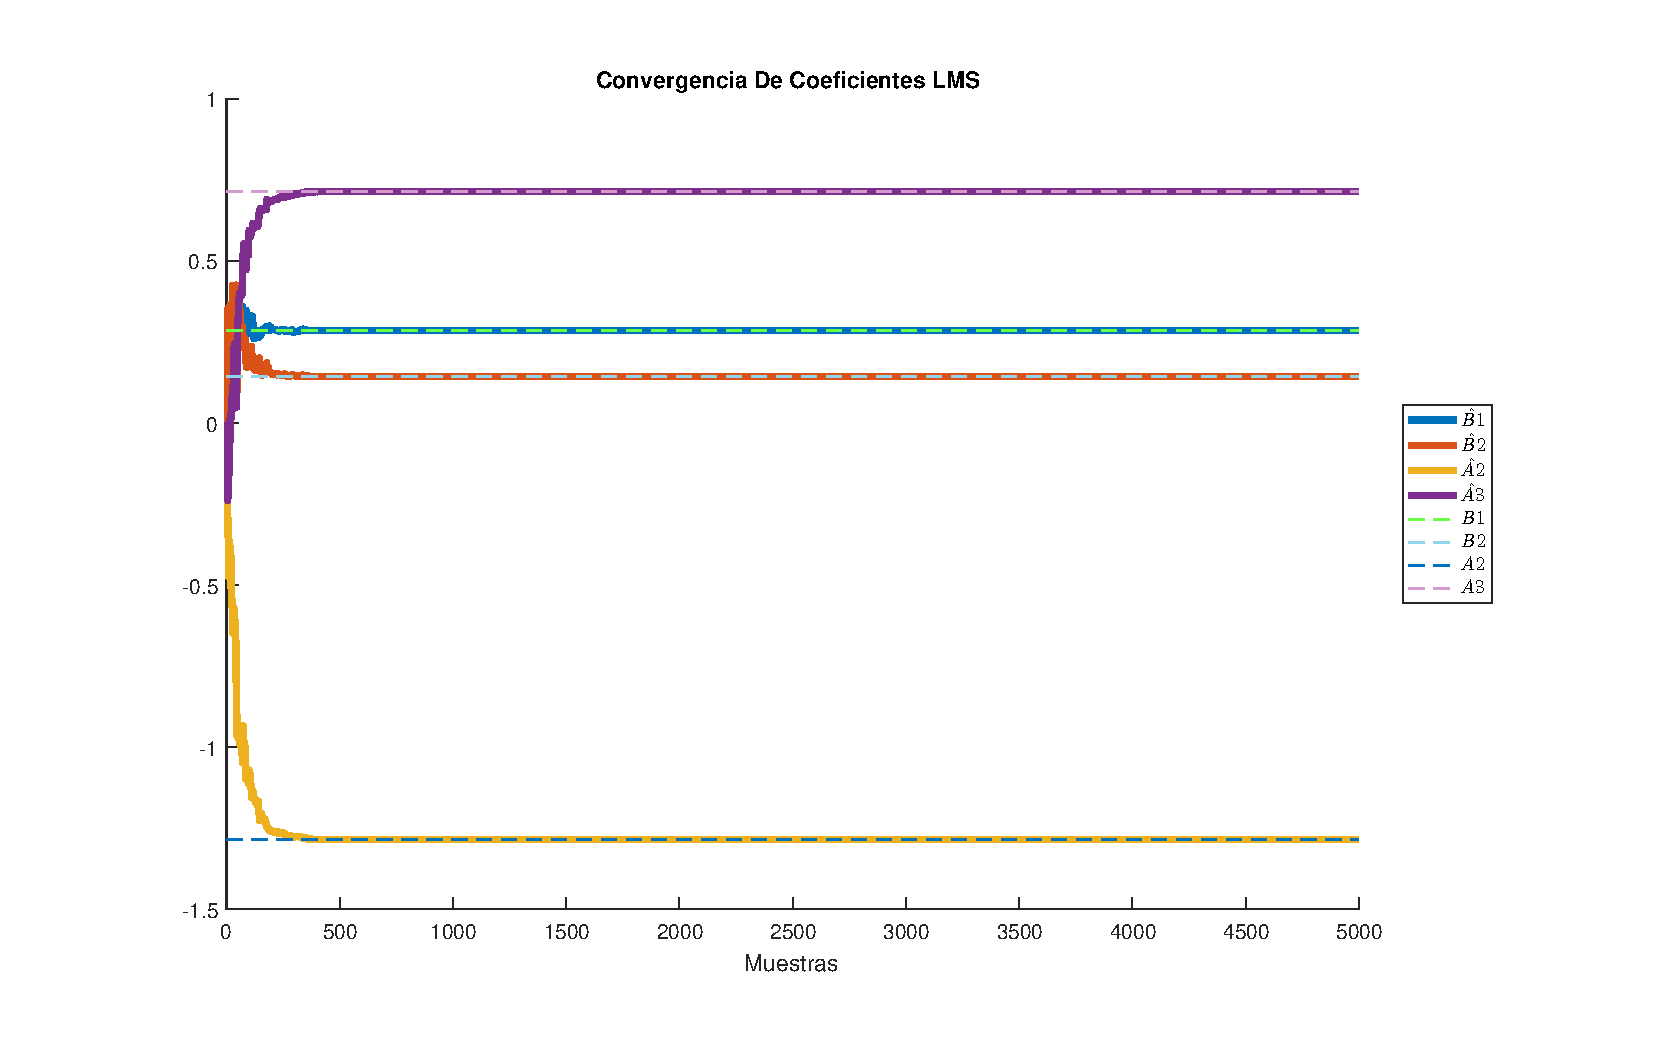
\includegraphics[width=1.0\textwidth, trim = 0cm 0cm 0cm 0cm]{graf_ej3.pdf}
		\caption{Convergencia de los coeficientes a partir de la estimación LMS.}
		\label{fig:ej3}
	\end{figure}

	\lstinputlisting[linerange=Resultados- ]{ej_3.m}
	Los resultados de la simulación a través de la función \texttt{solve()} se exponen en la siguiente tabla: \Juan{Correr el programa y completar porque no puedo yo}
		\begin{table}[h!]
			\centering
			\begin{tabular}{ccc}
				\toprule
				$m$	& $b$	& $k$\\
				\midrule
				&&\\
				\bottomrule
			\end{tabular}
			\caption{Resultados de la estimación de los parámetros.}
			\label{tab:res_ej3}
		\end{table}


